% ---------------- Title page texts ----------------
\newcommand{\BookTitle}{Road to RoboCup}
\newcommand{\BookSubtitle}{The Math Behind Neural Networks and\\ Soccer-Playing Robots\\[0.2em]--- Starting from the Basics}
\newcommand{\BookTagline}{A course for future RoboCup champions}
\newcommand{\BookAuthor}{Stella Alice Schlotter}

% ---------------- Answers: back | inline | off ----------------
%  back   = all answers collected in an appendix at the end of the book
%  inline = answers printed at the end of each chapter
%  off    = no answers (e.g. for a student version of a test)
\newcommand{\answermode}{back}

% ---------------- Packages ----------------
\usepackage[utf8]{inputenc}
\usepackage[T1]{fontenc}
\usepackage{mathpazo}
\usepackage[scaled=0.92]{helvet}
\usepackage{microtype}
\usepackage{amsmath,amssymb,amsthm}
\usepackage[a4paper,inner=2.8cm,outer=2.3cm,top=2.6cm,bottom=2.6cm]{geometry}
\usepackage{enumitem}
\usepackage[most]{tcolorbox}
\usepackage{xcolor}
\usepackage{tikz}
\usetikzlibrary{arrows.meta,positioning,calc}
\usepackage{pgfplots}
\usepgfplotslibrary{groupplots}
\pgfplotsset{compat=1.18}
\usepackage{etoolbox}
\usepackage{array}
\usepackage{subcaption}
\captionsetup{font=small,labelfont=bf,labelsep=period,hypcap=false}
\usepackage{graphicx}
\graphicspath{{images/}}
\usepackage{url}
\usepackage{fancyhdr}
\usepackage{titlesec}
\usepackage[hidelinks]{hyperref}

\setlength{\parindent}{0pt}
\setlength{\parskip}{0.6em}
\setcounter{tocdepth}{0}
\setcounter{secnumdepth}{1}

% ---------------- Colours ----------------
\definecolor{cupnavy}{RGB}{8,24,56}
\definecolor{cupgold}{RGB}{232,177,52}
\definecolor{cuppitch}{RGB}{18,110,60}
\definecolor{cupred}{RGB}{200,30,40}

% ---------------- Boxes and environments ----------------
\newtcolorbox{keyidea}[1][Key idea]{colback=blue!5,colframe=blue!60!black,fonttitle=\bfseries,title=#1}
\newtcolorbox{aibox}[1][Link to AI and robotics]{colback=green!5,colframe=green!40!black,fonttitle=\bfseries,title=#1}
\newtcolorbox{stepbox}[1]{colback=orange!6,colframe=orange!60!black,fonttitle=\bfseries,title=#1}

\numberwithin{figure}{chapter}
\theoremstyle{definition}
\newtheorem{definition}{Definition}[chapter]
\newtheorem{example}{Example}[chapter]

% ---------------- Math macros ----------------
\newcommand{\R}{\mathbb{R}}
\newcommand{\sig}{\sigma}
\newcommand{\dd}{\mathrm{d}}
\newcommand{\der}[2]{\dfrac{\dd #1}{\dd #2}}
\newcommand{\pder}[2]{\dfrac{\partial #1}{\partial #2}}
\newcommand{\vv}[1]{\mathbf{#1}}
\newcommand{\norm}[1]{\left\lVert#1\right\rVert}

% ---------------- Plot styles ----------------
% gr  : with axis labels x and y     grn : without axis labels
\pgfplotsset{
  gr/.style={
    width=7.2cm, height=6cm, axis lines=middle,
    xlabel={$x$}, ylabel={$y$}, grid=both,
    grid style={line width=0.1pt, draw=gray!30},
    major grid style={line width=0.2pt, draw=gray!50},
    tick label style={font=\footnotesize},
    legend style={font=\footnotesize, fill=white, fill opacity=0.85, draw=gray!50, text opacity=1},
    every axis plot/.append style={thick}, samples=100, enlargelimits=false
  },
  grn/.style={
    width=7.2cm, height=6cm, axis lines=middle, grid=both,
    grid style={line width=0.1pt, draw=gray!30},
    major grid style={line width=0.2pt, draw=gray!50},
    tick label style={font=\footnotesize},
    legend style={font=\footnotesize, fill=white, fill opacity=0.85, draw=gray!50, text opacity=1},
    every axis plot/.append style={thick}, samples=100, enlargelimits=false
  }
}

% ---------------- Chapter, part and section style ----------------
\titleformat{\chapter}[display]
  {\sffamily\bfseries}
  {\color{cupnavy}\fontsize{54}{54}\selectfont\thechapter\vspace{-0.2em}\color{cupgold}\rule{4cm}{2.5pt}}
  {0.6em}
  {\color{cupnavy}\Huge}
\titlespacing*{\chapter}{0pt}{-10pt}{26pt}
\titleformat{name=\chapter,numberless}[display]
  {\sffamily\bfseries}{}{0pt}{\color{cupnavy}\Huge}
\titleformat{\section}{\sffamily\Large\bfseries\color{cupnavy}}{\thesection}{0.8em}{}
\titleformat{name=\section,numberless}{\sffamily\large\bfseries\color{cupnavy}}{}{0pt}{}
\titlespacing*{\section}{0pt}{1.6em}{0.5em}
\titleformat{\subsection}{\sffamily\bfseries\color{cupnavy}}{\thesubsection}{0.8em}{}
\titleformat{name=\subsection,numberless}{\sffamily\bfseries\color{cupnavy}}{}{0pt}{}

\titleformat{\part}[display]
  {\sffamily\bfseries\centering}
  {\color{cupgold}\Large\MakeUppercase{Part}\ \thepart}
  {1em}{\color{cupnavy}\fontsize{30}{36}\selectfont}

% ---------------- Headers and footers ----------------
\newcommand{\currentchaptertitle}{}
\newcommand{\bookchapter}[1]{\chapter{#1}\gdef\currentchaptertitle{#1}}
\pagestyle{fancy}
\fancyhf{}
\renewcommand{\headrulewidth}{0.4pt}
\fancyhead[LE]{\sffamily\small\thepage\quad\textcolor{cupnavy}{\BookTitle}}
\fancyhead[RO]{\sffamily\small\nouppercase{\leftmark}\quad\thepage}
\fancypagestyle{plain}{\fancyhf{}\renewcommand{\headrulewidth}{0pt}\fancyfoot[C]{\sffamily\small\thepage}}

\makeatletter
\def\cleardoublepage{\clearpage\if@twoside\ifodd\c@page\else\hbox{}\thispagestyle{empty}\newpage\fi\fi}
\makeatother

% ---------------- Answer handling ----------------
\makeatletter
\newcommand{\collectedanswers}{}
\newcommand{\ansnum}{\thechapter}
\newcommand{\answerentry}[3]{%
  \renewcommand{\ansnum}{#1}%
  \section*{Chapter #1: #2}%
  \input{#3}%
}
\newcommand{\registeranswers}[1]{%
  \ifdefstring{\answermode}{inline}{%
    \section*{Answers to the practice problems}%
    \renewcommand{\ansnum}{\thechapter}%
    \input{#1}%
  }{%
    \ifdefstring{\answermode}{back}{%
      \protected@edef\@tmp@ans{\noexpand\answerentry{\thechapter}{\currentchaptertitle}{#1}}%
      \expandafter\g@addto@macro\expandafter\collectedanswers\expandafter{\@tmp@ans}%
    }{}%
  }%
}
\makeatother
\newcommand{\block}[1]{\addtocontents{toc}{\protect\par\protect\addvspace{3pt}\protect\noindent{\protect\sffamily\protect\small\protect\color{cupgold}\protect\textbf{#1}}\protect\par\protect\nopagebreak[4]}}
\newcommand{\includeplanned}[1]{\input{chapters/#1/chapter}}
\newcommand{\includechapter}[1]{%
  \input{chapters/#1/chapter}%
  \registeranswers{chapters/#1/answers}%
}

% ---------------- Title page ----------------
\newcommand{\makebooktitle}{%
\begin{titlepage}
\thispagestyle{empty}
\begin{tikzpicture}[remember picture,overlay]
  % background
  \fill[cupnavy] (current page.south west) rectangle (current page.north east);
  % pitch at the bottom
  \shade[top color=cupnavy, bottom color=cuppitch]
    ([yshift=1cm]current page.south west) rectangle ([yshift=8cm]current page.south east);
  \fill[cuppitch] (current page.south west) rectangle ([yshift=1cm]current page.south east);
  \begin{scope}
    \clip (current page.south west) rectangle ([yshift=8cm]current page.south east);
    \draw[white,opacity=0.28,line width=1.6pt] ([yshift=1.6cm]current page.south west) -- ([yshift=1.6cm]current page.south east);
    \draw[white,opacity=0.28,line width=1.6pt] ([yshift=1.6cm]current page.south) circle (3.2cm);
    \draw[white,opacity=0.28,line width=1.6pt] ([yshift=-2.5cm]current page.south) circle (6.5cm);
  \end{scope}
  % gold accent line
  \fill[cupgold] ([xshift=2cm,yshift=-3.2cm]current page.north west) rectangle ++(1.6cm,0.12cm);
  % texts
  \node[anchor=north west,text width=11cm,align=left,text=cupgold,font=\sffamily\bfseries\small]
    at ([xshift=2cm,yshift=-3.6cm]current page.north west) {\MakeUppercase{\BookTagline}};
  \node[anchor=north west,text width=13cm,align=left,text=white,font=\sffamily\bfseries\fontsize{58}{60}\selectfont]
    at ([xshift=2cm,yshift=-4.6cm]current page.north west) {\BookTitle};
  \node[anchor=north west,text width=10.5cm,align=left,text=white,font=\sffamily\Large]
    at ([xshift=2cm,yshift=-9.4cm]current page.north west) {\BookSubtitle};
  % robot
  \node[anchor=south east,inner sep=0pt]
    at ([xshift=-0.9cm,yshift=1.0cm]current page.south east)
    {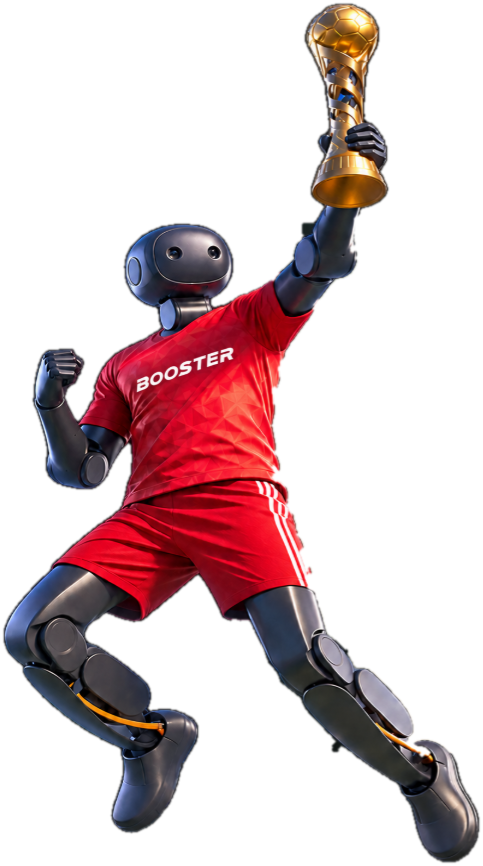
\includegraphics[height=18.5cm]{images/robot.png}};
  % author
  \node[anchor=south west,text=white,font=\sffamily\large,align=left]
    at ([xshift=2cm,yshift=1.2cm]current page.south west) {\BookAuthor};
\end{tikzpicture}
\end{titlepage}
}

\title{\BookTitle}
\author{\BookAuthor}
\date{}